

\begin{figure}
    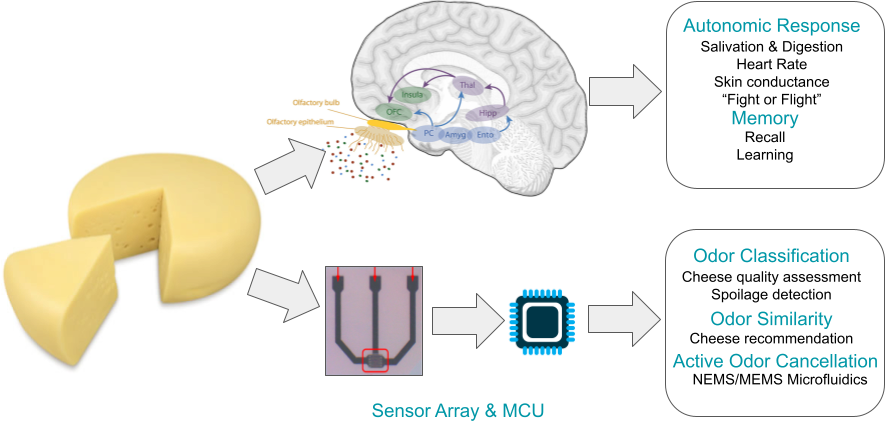
\includegraphics[width=\linewidth]{man_vs_machine.png}
    \caption{\small
        The human olfactory system transduces chemicals into electrical signals
        in the olfactory epithelium. Signals are then broadcast to a number of
        different parts of the brain, which enable autonomic nervous system
        responses, and can conjure memories and enable learning. This is
        mimicked in an odor sensor processor, where chemical sensor arrays
        transduce chemicals into odor signals which are sent to a compute
        element to execute odor related tasks.
    }
    \label{fig:man_vs_machine}
\end{figure}


Odor is a biological and psychological phenomenon (Figure~\ref{fig:man_vs_machine}) .  As such, chemical sensors
do not directly attempt to sense \textit{odors}, but rather to detect the
presence of \textit{chemical odorants}~\cite{dravnieks1985atlas,
snitz2019smellspace, keller2017predicting, malnic1999combinatorial}. A large
body of work has attempted to identify chemical-odor
relationships~\cite{snitz2019smellspace, keller2017predicting,
zhou2018hyperbolic, koulakov2011search, mamlouk2004dimensions}, e.g., 3-phenyl
propyl propionate has a `floral' odor, while (unsurprisingly) ethyl vanillin
has a `vanilla' odor~\cite{the_good_scents_company_2021}.  Thus, it is possible
to use chemical sensors to sense odors. Chemical sensors, such as metal-oxide
gas sensors, often operate on a basis of changes in electrical resistance in
reaction to the presence of one or more chemical analytes, with a higher
presence of the target analyte leading to larger changes in electrical
resistance.  However, these sensors are inherently noisy, as they will react to
the presence of chemicals suitably similar to their analyte (even if the
non-targeted chemical has a very different perceived odor).  Thus, a single
sensor is often inadequate for distinguishing between a quantity of its target
analyte, and a larger quantity of a non-target
analyte~\cite{schroeder2018carbon}. As such, commercial and academic
\textit{electric noses (e-nose)} use several sensors in a \textit{chemical
sensor array}.  The signals transduced by the sensor array is then fed into a
signal processing and/or machine learning algorithm in order to perform an
\olfc{} task, such as odor identification, odor pleasantness estimation, etc.

\begin{figure}[h]
    \centering
    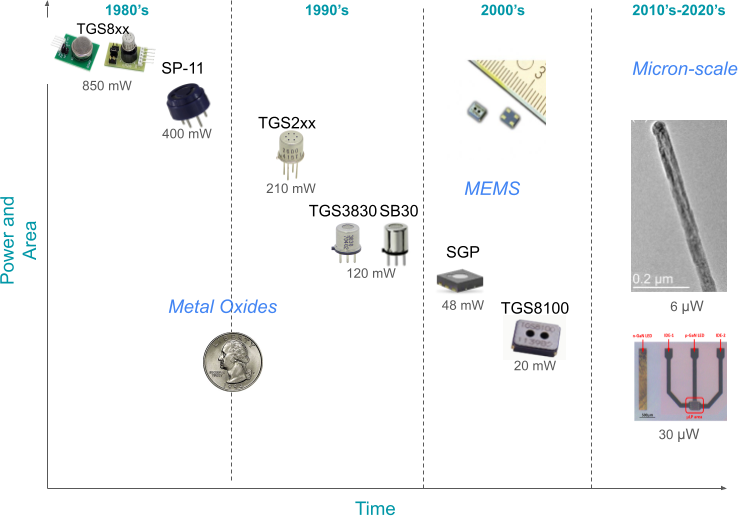
\includegraphics[width=0.7\linewidth]{sensor_timelines.png}
    \caption{\small
        Odor and chemical sensors continue to improve in power, area, and response
        times.
    }
    \label{fig:sensor_timelines}
\end{figure}


Fig.~\ref{fig:sensor_timelines} gives a high-level overview of the
development of chemical sensors used for \olfc{}.  Early sensors, which are
still commercially viable in products such as household smoke detectors, are
both physically large and high powered, as a result of requiring high operating
temperatures (often \(>\SI{500}{\celsius}\)). By greatly reducing the size of
the sensing surface, and thus the power required to heat the surface,
microelectromechanical systems (MEMS) lead to an order of magnitude decrease in
sensor power consumption. However, ultra low-power chemical sensors suitable for
\olfc{} have only come with the development of \si{\micro\meter} scale sensors
in the last decade. Nanowire chemical-resistive sensors enable room-temperature
flexible sensors in the low \si{\micro\watt} power
range~\cite{majhi2021recent}. In fact, recent work has shown self-powered
chemical sensors which exploit the piezoresistive effect of the sensing surface
when it reacts with an analyte~\cite{setiono2019real}. 

As discussed previously, previous work on olfactory processing has largely focused on sensing applications. No prior work addresses
the organization and design of the olfactory processor itself.



\begin{table}[]
\caption{Examples of olfactory applications and their constraints.}
\label{tab:applications}
\begin{adjustbox}{max width=\linewidth}
\begin{tabular}{@{}ll@{}}
\toprule
\textbf{Application}              & \textbf{Constraints}     \\ \midrule
Food Freshness Monitoring         & \(\leq\si{\milli\watt}\), lifetime of hours - months \\
Food Spoilage Detection           & \(\leq\si{\milli\watt}\), lifetime of hours - months \\
Personal Hygiene Monitoring       & low \si{\milli\watt}, lifetime of $\leq$ day         \\
Wearable Body Odor Detection      & low \si{\milli\watt}, lifetime of days               \\
Odor Biometric Authentication     & lifetime of months-years                             \\
Odor Biometric Forensics          & field deployable \& single use                       \\
Smart-Bandage infection detection & \(<\si{\milli\watt}\), lifetime of hours - days      \\
Air and water quality monitoring  & \(<\si{\milli\watt}\), lifetime of months - years    \\
Dangerous compound detection      & lifetime of days-years                               \\
Explosive detection               & lifetime of days-years                               \\
Gas Leak Tracing                  & requires spatial dispersed sensors, lifetime of minutes to hours \\
Odor Cancellation                 & requires odor synthesis  \\
Bespoke clothing deoderization    & requires odor synthesis  \\
Olfactory enabled xR              & requires odor synthesis \\
Food \& Scent recommendation      &                          \\
COPD \& Lung Cancer Screening     &                          \\
    \bottomrule
\end{tabular}
\end{adjustbox}
\end{table}


To build 
%programmable
olfactory computing systems, we must understand and analyze
the computational tasks underpinning odor-based applications. To identify a set of computation tasks that may be common across
a variety of odor-based applications, we surveyed 25 papers published in last 10 years on odor-based applications in Table~\ref{tab:applications} - at least one paper on each application was found. We identified the computational task(s) each paper was focused on. We also surveyed 10 odor-based electronic products in last five years and identified the corresponding computational task(s). Finally, we interviewed three olfaction experts and asked them for a list of computational tasks. We then created a list of tasks that appeared in at least two of the above three lists.

The tasks in our finalized list are
odor localization, odor classification, odor authentication, odor similarity,
active odor cancellation, odor pleasantness estimation, and odor demixing.

Odor classification, as the name suggests, is the task associated with
identifying the source of an odor.  Odor classification uses machine learning
and statistical techniques to map chemical sensor readings to source
odorants~\cite{kaeppler2013odor, husni2017odor}. Odor classification has many
commercial, industrial, agricultural, medical, and security applications,
including food and beverage monitoring for spoilage and quality 
%Assessed goods
%include 
%(e.g., teas
~\cite{yu2008quality, pan2014early},
%chen2013classification, yu2008identification,
%yu2009identification},
%alcohol~\cite{
%zhang2021channel,buratti2004characterization,shi2019deep
%},
%fruits~\cite{pan2014early, chen2018characterization, chen2018development,
%du2019ripeness, rasekh2021nose, %wu2017sensor}, cooking
%oils~\cite{karami2020application, teixeira2021application,
%rasekh2021classification}, meats and seafood~\cite{panigrahi2006design,
%wijaya2019noise, wijaya2021dwtlstm, aunsa2021electronic, grassi2022seafood},
%dairy~\cite{yang2021application, %labreche2005shelf}, and
%vinegar~\cite{li2022physicochemical, anklam1998characterisation}),
%. Industrial
%applications include
%\fi
environmental monitoring for air quality and air pollution
estimation~\cite{caron2019identification, szulczynski2017different,
tacstan2019real, de2008tinynose}, 
%while agriculture applications include
waste-water monitoring and forestry applications~\cite{wilson2013diverse,
blanco2018development, lagod2019application, dewettinck2001electronic},
%. Medical
%applications for odor classification have begun to emerge, including 
hygiene
monitoring~\cite{lorwongtragool2014novel}, diagnosis of lung diseases such
as COPD and lung cancer~\cite{gardner2000electronic, va2021noninvasive,
binson2021discrimination, d2010investigation},
%.  Security applications include
and explosive device detection~\cite{brudzewski2012metal, lopez2017electronic,
sun2013liquid}. Odor classification is performed with a variety of machine
learning and statistical analysis techniques such as principal component
analysis (PCA), support vector machines (SVM), artificial neural networks
(ANN), and K-Means cluster analysis (KMeans).

Biometric authentication using odor, or, odor authentication, is the olfactory
equivalent of fingerprint, facial, iris, or voice authentication techniques
which are currently in vogue on mobile devices~\cite{stokkenes2016biometric}.
Individual humans have an identifiable scent due to genetic and environmental
factors~\cite{penn2007individual}, and many studies have shown successful
discrimination of individuals' body odor using chemical sensor
data~\cite{wongchoosuk2009detection, jha2015quick, jha2016gc}. Several odor
authentication schemes have been proposed~\cite{yang2018human,
shu2014identification}. Odor authentication is similar to odor classification
in that it uses machine learning to classify a body odor as authenticated or
non-authenticated, however, it typically uses a dictionary of known odors.
Similar to other biometric authentication techniques, odor authentication
consists of first extracting features from chemical sensor data, often using
parametric machine learning learning techniques, and then comparing those
features to a user dictionary. Thus, new authenticated users can be enrolled
and old users removed without needing to retrain a new model from the ground
up~\cite{wong2001enhanced}. Algorithms in odor authentication include PCA, SVM,
ANN, K-Means, and KNN.

In the odor similarity task, the goal is to estimate the odor similarity of two
different chemical mixtures.  Traditionally, this has been done by first
identifying the chemical structure of the mixtures' constituent chemicals via
\gcms{}
% NOTE: Footnotes are not allowed in NSF Project Description
(However, it can also be done with sensor data).  These
chemical structures are then mapped to fixed length vectors from an inner
product space, and then the mixtures are represented by weighted sums of the
constituent chemical vectors.  Finally, the similarity of the two chemicals is
scored based on the angle between the two vectors
(AngleDist)~\cite{snitz2013predicting}. %Odor similarity can power an odor
%recommendation engine, in which a new odor is suggested to users based on
%similarity to a known odor the user finds pleasant.

Active odor cancellation is the olfactory equivalent of active noise
cancellation.  Active odor cancellation attempts to `block out' one or more
malodors in an environment by \textit{adding} odors which cancel the malodor,
rendering it as olfactory white noise~\cite{varshney2014active}.
The algorithm which determines how much of each odor to add to the environment
consists of solving a quadratic program which, in many cases, is convex. As
such, gradient descent based optimizers may be used to find local, and often,
global solutions to the optimization problem.

The pleasantness of an odor is highly dependent on the physical properties of
the odorant molecular structure~\cite{arshamian2022perception}. As such, odor
pleasantness estimation is assigning a value (either numeric or categorical) to
a chemical corresponding to its predicted pleasantness.  This has been achieved
using PCA and SVM~\cite{li2018accurate, li2020perception, shang2017machine}.

Odorants exist in mixtures, including time-evolving mixtures, yet often only
one chemical odorant is of interest.  Odor demixing is the task which isolates
the signal corresponding to the chemical of interest.  
This can be achieved
using \gcms{}, however, as \gcms{} requires a large laboratory set-up, and
takes twenty or more minutes to perform. %different techniques are required when
%working with low-power chemical sensors. 
There have been a number of works
which attempt to tackle this problem in context of low-power chemical sensors~\cite{maho2021real, victor2014combining,
fonollosa2014chemical}, but odor demixing remains a largely unexplored \olfc{}
task. However, odor demixing has been studied in biological olfactory systems,
and several studies have proposed biology inspired compressive sensing, which
enables reconstructing sparse signals from many fewer samples than is typically
required (e.g., in an audio setting, from samples taken below the Nyquist
rate)~\cite{fornasier2015compressive}. Compressive sensing, namely, orthogonal
matching pursuit (OMP), has been shown to be useful in the olfactory domain
since individual odors are sparse within the large space in which an odor can
be represented.

Odor localization is the task of identifying the source location of an
odorant `plume' within an environment.  Odor localization is efforts are
exacerbated by the turbulent nature gas plumes which result in non-convex
distributions of the odarant plume with local maxima, which limit the
applicability of gradient based methods.  As such, biology inspired methods, as
well as probabilistic methods such as particle filtering are commonly used in
conjunction with a model of plume dynamics~\cite{vickers2000mechanisms}.
While odor localization
%is unique
%among the tasks in that it 
is typically performed by either a mobile field robot~\cite{chen2019odor}, or
by a distributed sensor network~\cite{hayes2002distributed}, as odor
localization benefits from taking chemical readings in multiple locations
throughout the environment, we also consider future applications where a
wearable aids a moving human or an animal in identifying an odor source (gas
leak or fire source, for example).
%Analogously, consider triangulating a radio signal broadcast
%location --- this task is much easier with receivers in multiple locations than
%with only a single radio receiver.  Indeed, with only a single, fixed chemical
%sensor, it is exceedingly difficult to determine if a faint signal is due
%to a strong odorant source far away, or a weak odorant source nearby.


%\subsection{Algorithms}

 
We will implement the above tasks as a bona fide olfactory computing benchmark suite --- OlfacSuite --- by
    porting all benchmark code to C and OpenMP, designing representative inputs
    for each benchmark, and providing baselines on existing systems. OlfacSuite --- software, data, \& build scripts --- as well as
    executable binaries for major platforms --- will be published under
    an open source license in order to enable commercial and academic
    research into olfactory computing.Data and inputs will be drawn from published real
    world samples.
    
    OlfacSuite will be published with a CMake based build system.  As CMake
    is an open-source, cross platform build automation tool targeting all
    major operating systems, and since nearly all computer architectures
    have open source or proprietary C compilers, researchers will be able
    to get OlfacSuite running on a wide variety of systems quickly and easily.
    For major architectures (e.g., ARMv7, ARMv8, x86\_64, i686, etc.),
    we will provide prebuilt OlfacSuite binaries.



\begin{figure}
    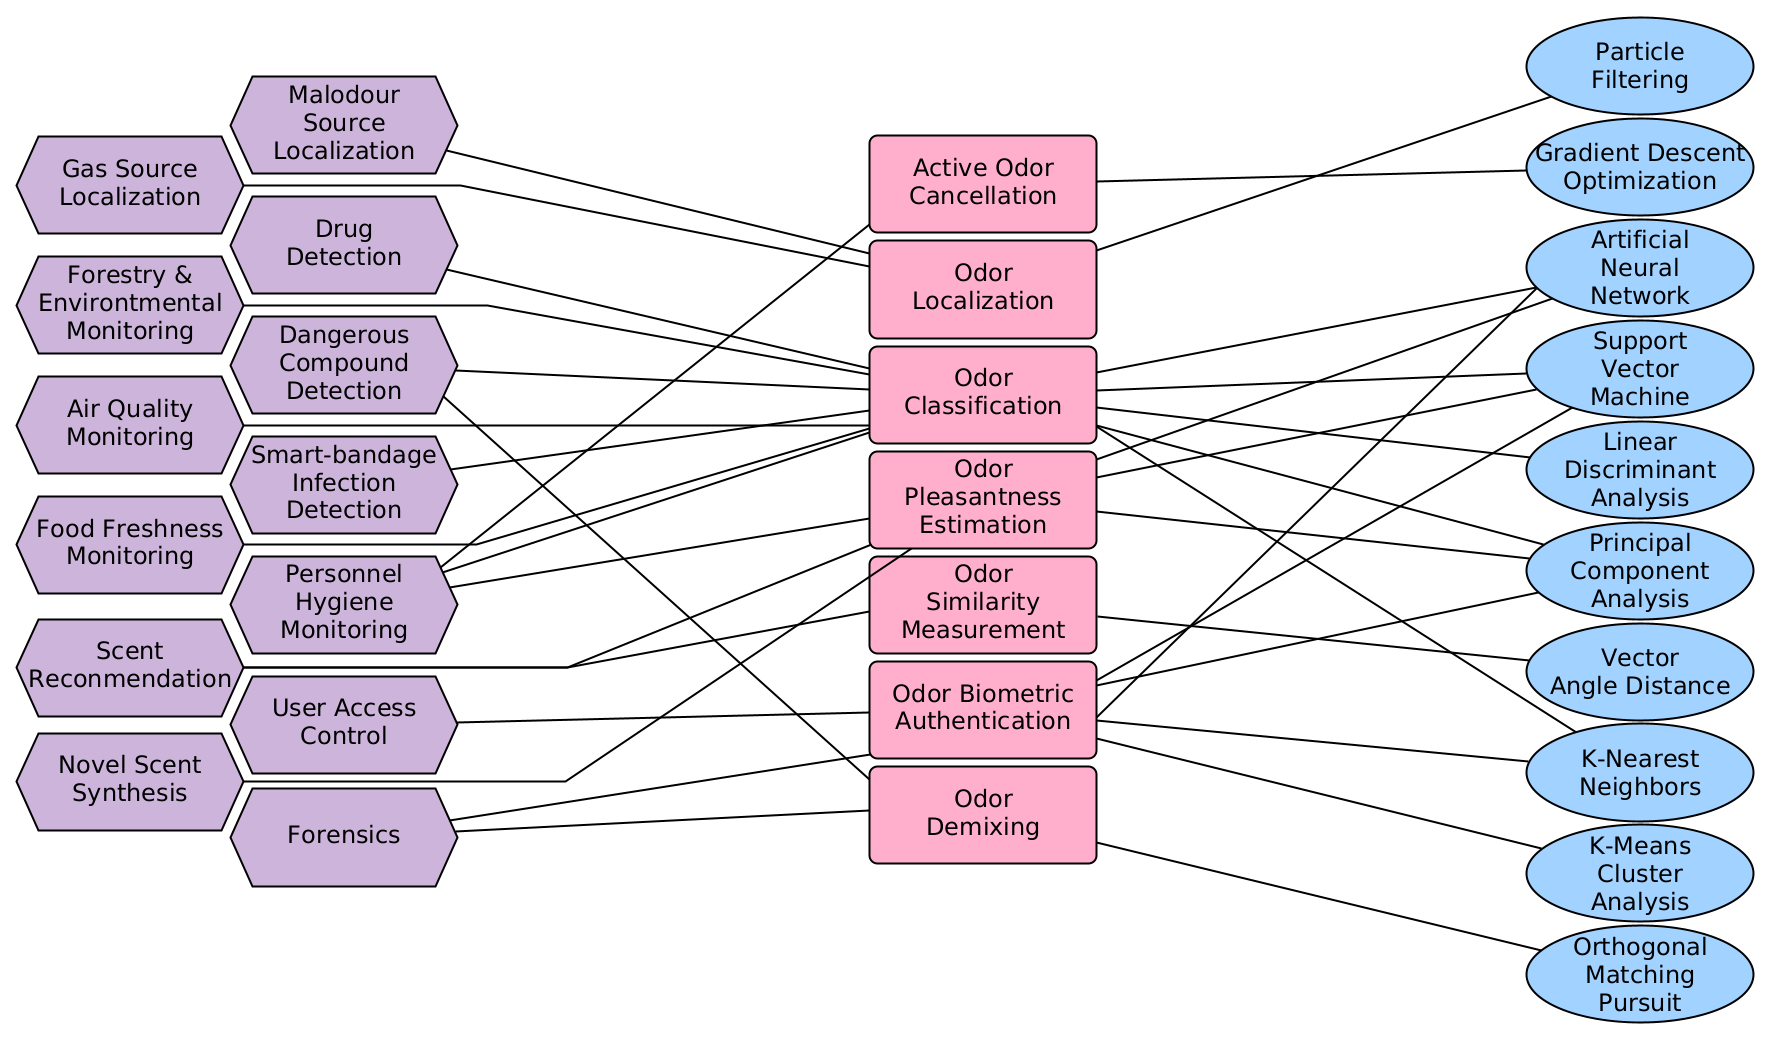
\includegraphics[width=\linewidth]{app_task_kernel.png}
    \caption{
        \small Graphical depiction of relationship between applications
        (\textcolor{purple}{hexagons}) which are composed from tasks
        (\textcolor{pink}{rectangles}).  Tasks are implemented using a
        computational kernel (\textcolor{blue}{ellipses}). Some tasks can be
        supported by multiple kernels.
    }
    \label{fig:app_task_kernel}
\end{figure}

% \input{tables/applications}

To analyze a computer architecture's performance on olfactory workloads, a
diverse and representative collection of olfactory algorithms underpinning the
odor computational tasks is needed.  Fig.~\ref{fig:app_task_kernel} is a graphical depiction of the relationship
between olfactory applications (hexagons), the tasks (ellipses) from which the
applications are composed, and the computational kernels (rectangles) which can
be used to implement the task.  Some tasks may be implemented using one of
several kernels, such as odor classification which can be supported by several
machine learning and statistical analysis techniques. 
%Below we describe the nuances of implementation of the
%identified computational kernels in context
%of \olfc{}.

The algorithms themselves may have olfaction-specific implementation and input characteristics.
For example, particle filtering may require a dynamical model of the
odorant plume.  
Due to the slow rate at which odorant mixtures change,
the number of data points, $d$, in the Principal component analysis for olfactory
applications is limited to the low hundreds,
while the number of sensors in a sensor array is often less than ten.
Thus PCA requires normalizing only a small number of distributions with
a small number of samples, and performing eigen decomposition on a small
correlation matrix.  Similarly, in the odor context, finding the
principal components of an sensed input requires only multiplying the input
by a small $n\times n$ matrix.
Linear discriminant analysis for olfactory applications is extremely light weight,
with time and space complexity quadratic  and linear, respectively,
in the number of sensors in the sensor array.
In olfactory computing, the input
sample is a vector of sensed values from the chemical sensor array. Thus, the
complexity of running the support vector machine is the same as computing the
principal components or linear discrimnants of the input.  
The most prominent type of Artificial neural networks (ANN) seen in olfactory computing is the multilayer
perceptron (MLP), in which each layer is fully connected. The input to the
MLP is typically the sensed data directly, with no preprocessing steps
involved (consider, for example, that there is no need for pre-processing
to help the model learn high-frequency content, as there is in image and audio
processing, since odor signals typically lack high frequency content).
The MLPs used in \olfc{} tend to be just barely deep - often with
only a single hidden layer - and with very few neurons (often $< 50$).
Termination of Kmeans algorithm is known to be NP-Hard~\cite{aloise2009np}.  In practice,
for odor processing, KMeans often terminates quickly~\cite{yang2018human,
zheng2019wearable}.

We make several observations about the computational characteristics of the kernels that may impact any architecture we build for these workloads.
First, none of the
kernels are integer kernels --- all kernels require fixed-point arithmetic.
Thus hardware support for fixed-point operations is necessary for energy
efficient computation of olfactory workloads.
Second, none of the kernels require complex numbers --- this is very different
than audio and image sensor processing which makes copious use of classical
frequency domain signal processing algorithms~\cite{mandic2007complex, paris2011local}.
Unlike hearing and sight, which arise from sensing wave-based phenomena
(i.e., light and pressure waves),
the sensation of odor arises from sensing non-wave chemicals.  Thus, there
is no frequency or phase component to the sensed odor signal. Principal
component analysis (PCA) does include computing eigenvalues, but since
correlation matrices are symmetric, the eigenvalues are necessarily real
valued.  Thus hardware support for complex arithmetic and fast Fourier transform
is not required.
Third, the primary arithmetic primitives are multiplication and addition, often
in the form of multiply-accumulates needed for evaluation of linear functions,
as found in ANN, SVM, LDA, PCA, AngleDist, and OMP.  Although many kernels use
non-linear operations, these operations are often either multilinear (i.e.,
multiplication of variables rather than variables by fixed constant), or are
limited in number relative to multiplications and additions, and they are
temporally isolated between long sequences of linear and multilinear
operations.
%\footnote{Due to the computational simplicity of reLU activations,
%we ignore these in analysis of non-linear vs linear interspersedness.}  
Thus,
dedicated hardware to accelerate linear operations is likely to provide
significant benefits for olfactory application workloads.
Fourth, there is a large spread in working set size among kernels, with some
kernels having very small working sets which can be supported by a very small
data memory, or even with a large register file, while several kernels require
significantly more data memory.  In fact, kernels such as PF can be made
to require drastically more memory by increasing the number of particles used
in its Monte Carlo simulation, which can lead to better localization accuracy.
This wide range in memory requirements suggests that a scalable memory
organization is likely to provide energy and power benefits for olfactory
applications.
Fifth, many of the tasks support vectorization, even auto-vectorization, which
indicates that parallel architectures are likely to perform well on olfactory
application workloads.
%These kernel characteristics are summarized
%in Table~\ref{tab:kernels}, with data derived from analysis of implementations
%of the kernels for a scalar CPU with packed SIMD ISA extension.

Based on the above observations, we will explore architectures for olfactory processing. 
Olfactory computing is applicable in many application domains. However, in many
domains, the light computational requirements of its algorithmic primitives
means the attention of architects is little needed. XR headsets, able to power
high resolution 3D graphics, for example, will have little trouble running
olfactory computing tasks.  There are, however, application domains with
extreme constraints which make olfactory computing interesting to architects.
Form factors such as wearables, (earrings, pendants, brooches, etc), bandages
(e.g., for detecting infections), adhesives (e.g., for body odor monitoring),
packaging (e.g., smart packages that detect food spoilage), swabs (for breath,
urine, body fluids-based diagnostics, for example), sensors-in-the-wild ( e.g.,
air quality monitoring, surface and ground water quality monitoring), etc., may
only allow for energy harvesting.  Field deployed sensors may need to maximize
limited battery energy capacities over long periods, or be self-powered.  In
these domains, both power and energy are stringent limitations.

 
%Fig.~\ref{fig:arch} presents an overview of \arch{}.
%\arch{}'s aim is to support energy efficient \olfc{}, given the
%lax performance requirements of \olfc{} applications, and the
%constrained energy budget available to edge devices.  Thus, \arch{} is designed
%for operating points at below nominal voltage.

\begin{figure}
\centering
    
\includegraphics[width=\linewidth]{arch_odor.png}
    \caption{\small
            An example organization of olfactory computing processor as an MCU with Vector-MAC-unit and CGRA
            accelerators. Since the processor aims for energy efficiency, achieved by
            operating at low voltage and frequency, the processor exploits the lack
            of voltage scaling available to SRAMs to enable multiple SRAM
            accesses on a single port per clock cycle.
        }
    \label{fig:arch}
\end{figure}

An example architecture of a programmable
ultra-low-power olfactory computing hardware platform supports low frequency
and voltage operation; programmability is supported to lower costs and to
maintain generality in a domain where applications are likely to evolve.  Our preliminary
architecture (Fig.~\ref{fig:arch}), is a heterogeneous reconfigurable
odor monitoring and analysis architecture consisting of a \SI{32}{\bit} 
MCU with two integrated accelerators, both supporting fixed-point
operations. 
The first accelerator is a \SI{128}{\bit} packed SIMD unit which accelerates
fixed-point fused muliply accumulate operations on 4, 8, 16, and \SI{32}{\bit}
datatypes, to support the copious multiply-accumulates found in ANN, SVM,
LDA, PCA, VAD, and OMP algorithms.
Unlike a typical packed SIMD ISA extension, the processor's vector-multiply-accumulate unit does not have an
additional SIMD register file.  Instead, data is accessed directly from memory,
which is made possible by the discrepancy between the core voltage at the
minimal energy operating points of processor, and the
SRAM's nominal voltage required to ensure memory retention. Additionally,
since the size of data memory required by many olfactory applications
is small, the overhead of a dedicated SIMD register file may be large relative
to data memory in its entirety.
The second accelerator is a coarse-grained
reconfigurable streaming dataflow architecture with several heterogeneous PEs
(adder PEs, and multiply-accumulate PEs) arranged in a grid, and
utilizing a bufferless, single-cycle, multi-hop routing network, as
in~\cite{wang2019hycube, gobieski2021snafu}. Each PE contains a small
(\SI{16}{\byte}) buffer, in which it can store model parameters, as well as
accumulated sums. PEs are capable of \SI{32}{\bit} width packed-SIMD
execution of multiplies and adds (i.e., $1\times$ \SI{32}{\bit} operation,
$2\times$ \SI{16}{\bit} operations, etc.).  The dataflows supported  on
the CGRA enables mapping convolution layers with various kernel sizes and strides.
This is important as although currently most olfactory ANNs are MLPs,
there do exist CNNs for olfactory applications, and the choice of the best
model for olfactory tasks is still being litigated.
Both accelerators support efficient packed SIMD addition and multiplication for
datatypes of varying width, as wide adders and multipliers can be
recursively built from narrow adders and multipliers.
Wide adders are built from narrow adders via carry-out propagation.

We will explore other computer architectures as well for olfactory processing
targeting wearable and distributed sensor networking olfactory applications.
Many ultra-low power candidate architectures currently exist, including
ultra-low power microcontrollers~\cite{heller2019microwatt} and GPUs~\cite{},
as well as \(<\si{\milli\watt}\) spatial
architectures~\cite{kersey2017lightweight}. Preliminary results analyzing
olfactory applications and their computational requirements  show that, for
many applications, performance requirements are lax, and absolute computational
and memory requirements are low.  This suggests that the architectural design
space considered must go beyond looking at just computer organization and
design, but must encompass memory design and operating points. Due to lax
performance requirements and low computational requirements, olfactory
computing is likely a strong candidate for near or sub-threshold
computing~\cite{raychowdhurry2005computing}. Thus the design space exploration
will include amenability to and impact of voltage scaling into the near and
sub-threshold regions. Although this type of work has been done for CPU and GPU
based architectures, it has, to the best of our knowledge, never been done for
reconfigurable spatial architectures. Also, as many olfactory applications
require very small amounts of data memory, memory design will be an important
aspect of the design space exploration.  The size, geometry, and number of SRAM
banks will be explored.  Additionally, since some applications require trivial
amounts of data memory, we will also consider memories composed wholly or
partially out of latches and flip-flops, rather than SRAM cells. Although SRAM
cells are typically smaller and consume less power than flip-flops and latches
at nominal voltage, SRAM cells are generally not ammenable to voltage scaling.
Thus, at low voltages, latch and flip-flop based memories may consume less
power than an equivalently sized SRAM.

We will also prototype and test an olfactory processing chip in TSMC \(\leq
\SI{65}{\nano\meter}\) technology. The candidate design, the heterogeneous
architecture described above, provides ample opportunities for architecture and
physical design innovations in order to minimize energy of the prototype chip,
especially since near-threshold processing would be involved. PI Kumar teaches
a chip tapeout class every year where several RISC-V-based SoCs with a
microcontroller core and multiple accelerators have already been taped out and
tested successfully. The experience and the resources would be leveraged in the
proposed prototyping effort.

Testing sub-objectives include olfactory system design and PCB design, porting
OlfacSuite applications to the chip, and collecting measured OlfacSuite
results.  System design will incorporate multiple odor sensors and a hardware
debug system. Porting OlfacSuite applications to the chip requires annotating
the OlfacSuite C code with pragmas which enable the architecture's compiler to
automatically generate configurations and data streams for its spatial
accelerator.
       
Finally, we will also analyze both proposed and existing olfactory computing
hardware in a heterogeneous, networked computational setting, in which
computation can be offloaded from the olfactory device onto a number of other
devices, including smart watches, smart phones, and high performance cloud
systems. The work will be analogous to what was described earlier in context of
earables.


